\documentclass[10pt,letterpaper]{article}
\usepackage[top=0.85in,left=2.75in,footskip=0.75in,marginparwidth=2in]{geometry}

% use Unicode characters - try changing the option if you run into troubles with special characters (e.g. umlauts)
\usepackage[utf8]{inputenc}

% clean citations
\usepackage{cite}

% create filler text
\usepackage{lipsum}

% hyperref makes references clicky. use \url{www.example.com} or \href{www.example.com}{description} to add a clicky url
\usepackage{nameref,hyperref}

% line numbers
\usepackage[right]{lineno}

% improves typesetting in LaTeX
\usepackage{microtype}
\DisableLigatures[f]{encoding = *, family = * }

% text layout - change as needed
\raggedright
\setlength{\parindent}{0.5cm}
\textwidth 5.25in 
\textheight 8.75in

% Remove % for double line spacing
%\usepackage{setspace} 
%\doublespacing

% use adjustwidth environment to exceed text width (see examples in text)
\usepackage{changepage}

% adjust caption style
\usepackage[aboveskip=1pt,labelfont=bf,labelsep=period,singlelinecheck=off]{caption}

% remove brackets from references
\makeatletter
\renewcommand{\@biblabel}[1]{\quad#1.}
\makeatother

% headrule, footrule and page numbers
\usepackage{lastpage,fancyhdr,graphicx}
\usepackage{epstopdf}
\pagestyle{myheadings}
\pagestyle{fancy}
\fancyhf{}
\rfoot{\thepage/\pageref{LastPage}}
\renewcommand{\footrule}{\hrule height 2pt \vspace{2mm}}
\fancyheadoffset[L]{2.25in}
\fancyfootoffset[L]{2.25in}

% use \textcolor{color}{text} for colored text (e.g. highlight to-do areas)
\usepackage{color}

% define custom colors (this one is for figure captions)
\definecolor{Gray}{gray}{.25}

% this is required to include graphics
\usepackage{graphicx}

% use if you want to put caption to the side of the figure - see example in text
\usepackage{sidecap}

% use for have text wrap around figures
\usepackage{wrapfig}
\usepackage[pscoord]{eso-pic}
\usepackage[fulladjust]{marginnote}
\reversemarginpar

% document begins here
\begin{document}
\vspace*{0.35in}

% title goes here:
\begin{flushleft}
{\Large
\textbf\newline{Elucidating the Role of Complement in Opioid Use Disorder Reward Pathways}
}
\newline
% authors go here:
\\
Aum Champaneri\textsuperscript{1,$\dagger$},
Jessy Alexander\textsuperscript{1, $\dagger$, *}
\\
\bigskip
\bf{1} Department of Biochemistry
\\
\bf{2} Department of Medicine, Division of Nephrology
\\
\bf{$\dagger$} Jacobs School of Medicine and Biomedical Sciences, SUNY University at Buffalo, Buffalo, New York
\bigskip
\\
* \href{mailto:jessyale@buffalo.edu}{jessyale@buffalo.edu}

\end{flushleft}

\section*{Abstract}
Opioid use disorder (OUD) is characterized by compulsive opioid consumption and associated neuroinflammatory changes. The complement system, a key component of the innate immune response, has been implicated in OUD, however, its role remains incompletely understood. In this study, we utilized publicly available single-nucleus and bulk RNA sequencing datasets to assess the expression patterns of complement proteins—C3, Factor H (FH), C3aR1, and C5aR1—in the caudate nucleus, putamen, dorsolateral prefrontal cortex, and nucleus accumbens of both naïve and OUD individuals. Uniform Manifold Approximation and Projection (UMAP) analyses revealed distinct cellular clusters within these brain regions. Spatial expression patterns indicated that FH is predominantly expressed in endothelial cells, whereas C3, C3aR1, and C5aR1 are significantly expressed in microglia. Notably, microglial expression of these complement components exhibited sex-specific differences, with different clusters showing higher expression levels in females than males. Furthermore, microglial populations from naïve and OUD individuals were distinguishable, suggesting differential activation states associated with OUD. These findings provide novel insights into the cellular and molecular alterations in the brain associated with OUD, highlighting the complement system's potential involvement in this setting. The observed sex-specific differences in complement protein expression underscore the importance of considering biological sex in neuroimmune research and therapeutic strategies targeting the complement system in OUD.

% now start line numbers
\linenumbers

% the * after section prevents numbering
\section*{Introduction}

Opioids are among the most widely prescribed analgesics globally \cite{vanAmsterdam2015}. Due to their high rewarding activity, opioids are abused \cite{SAMHSA2018, Seth2018}, leading to the opioid use disorder (OUD) crisis, characterized by its widespread prevalence and profound clinical and societal implications. Reward is a central nervous system (CNS) process that arises when an individual’s basic drives—such as hunger and thirst are fulfilled \cite{Fields2015}. From an evolutionary standpoint, the sensation of reward reinforces these behaviors, encouraging individuals to repeat these actions \cite{Fields2015}. Research has identified the ventral tegmental area (VTA) and the nucleus accumbens (NAc)—key components of the mesolimbic pathway—as critical regions involved in processing reward-related stimuli, \cite{Volkow2015} (Figure \ref{Brain}).

\begin{figure}[ht] %s state preferences regarding figure placement here
% \centering
\includegraphics[width=1.00\textwidth]{BrainArea.jpg}
\caption{\color{Gray}\textbf{Schematic of Brain Areas in Dataset. }
\texttt{GSE225158} contains snRNA-seq data from the Caudate and Putamen. \texttt{GSE174409} contains Bulk RNA-seq data from the Dorsolateral Prefrontal Cortex (DLPFC) and Nucleus accumbens (NAc). DLPFC is central to executive function and is critical to new learning when working memory and attention are necessary \cite{ZGALJARDIC2010458}. The putamen, caudate, and nucleus accumbens make up the striatum. The striatum sends inputs to the basal ganglia and is essential for voluntary movement control \cite{Hikosaka2000}| is also activated by rewards in social situations \cite{Baez2013} and is involved in goal-directed behaviours. Striatal dysfunction is linked to psychiatric disorders| including OUD \cite{Phan2024}.
}
\label{Brain} % \label works only AFTER \caption within figure environment
\end{figure}

While the primary focus has been on the pharmacological effects of opioids on neuronal signaling and reward pathways, emerging evidence highlights the significant role of neuroinflammation in the pathophysiology of OUD. Central to neuroinflammation is the complement system, a key component of innate immunity has emerged as a critical modulator of neural and inflammatory responses to opioid exposure. The complement system (Figure \ref{ComplementCascade}), a powerful arm of the innate immune system, consists of over 40 plasma and membrane-bound proteins that are activated through three activation pathways: classical, lectin, and alternative pathways. These cascades converge to generate effector molecules that mediate pathogen opsonization, inflammatory cell recruitment via anaphylatoxins (e.g., C3a, C5a), and direct microbial lysis through the membrane attack complex (C5b-9). Beyond its traditional role in pathogen clearance, the complement system regulates synaptic pruning during neurodevelopment and modulates adaptive immunity by enhancing B-cell antibody production and T-cell activation. Notably, its activation products influence neuroimmune crosstalk by interacting with glial cells and neurons, potentially shaping neuroinflammatory states implicated in addiction pathways. This dual role in peripheral immunity and central nervous system plasticity positions the complement system as a critical mediator of immune –brain interactions relevant to substance abuse disorders. Our studies showed that chronic opioid use, such as heroin abuse, exacerbates neuroinflammation, especially in individuals with co-occurring HIV-1 infection. In these cases, increased expression of complement components like C1q, SC5b-9, C5aR, and C3aR was observed in postmortem brain tissues, highlighting that complement activation may play a proactive role in shaping neuroimmune responses to chronic opioid exposure \cite{Mahajan2017}. However, the intersection of gender, complement signaling, and OUD remains incompletely understood. This gap is particularly critical given the emerging links between complement signaling, synaptic pruning, and addiction-related neural plasticity and accumulating evidence that males and females differ in their behavioral responses to opioids, relapse risk, and treatment outcomes.

\begin{figure}[ht] %s state preferences regarding figure placement here
%\renewcommand{\thefigure}{2}
% \centering
\includegraphics[width=1.00\textwidth]{ComplementCascade.jpg}
\caption{\color{Gray} \textbf{Complement Activation Pathways. }
The classical pathway is activated by antigen/antibody complexes, recognized by C1q in complex with C1r and C1s \cite{Girardi2020}| then forming C3 convertase (C4b2a). The lectin pathway is initiated by the binding of mannose-binding lectin with mannose residues on pathogen surfaces, which activates mannose-associated serine proteases (MASPs) to form the same C3 convertase (C4b2a) \cite{jcm10102188}. The alternative pathway is triggered by antigens and is also spontaneously auto-activated| this also leads to the formation of C3 convertase (C3bBb). The C3 convertase's hydrolyze C3 to yield C5 convertase's (C4b2bC3b \& C3bBbC3b). These pathways terminate with the generation of C5b-9 or MAC (Membrane Attack Complex).
}
\label{ComplementCascade} % \label works only AFTER \caption within figure environment
\end{figure}

Historically, men exhibit higher rates of opioid abuse, yet women demonstrate accelerated progression to dependence, greater susceptibility to addiction, and increased risk of overdose. Recent proteomics studies reveal significant changes in 15 circulating plasma proteins in females that is modulated by estradiol, including factor B, complement 4, precursor (C4), C-reactive protein (Crp), and serine peptidase inhibitor 3L (Serinpa3l). Opioid using surgery patients had reduced C4bpA, and enhanced expression of factor D in circulating leukocytes (WBCs) in opioid-consuming patients. Complement therapeutics is gaining momentum and complement proteins also play a critical role in local homeostasis. Therefore it is important to investigate the role of complement proteins in this setting and their impact on sex-specific differences in OUD pathology. Traditional bulk transcriptomic approaches often obscure cell-type specific responses, limiting insights into heterogeneous immune and neural populations. Single-nucleus transcriptomics (snRNA-seq) enables high-resolution profiling of transcriptional dynamics across individual cells, revealing nuanced cellular adaptations to chronic opioid exposure. This technology offers a powerful approach to investigate how complement gene expression is regulated in a sex-specific manner across distinct neural and immune cell populations in the context of OUD. By leveraging single-nucleus RNA sequencing (snRNA-seq), we can identify cell-type-specific and sex-specific alterations in complement component and receptor expression, uncovering novel insights into the molecular landscape of opioid-related neuroinflammation.

Despite the growing recognition of neuroinflammation in OUD, and the direct evidence linking complement proteins to OUD, the specific contributions of the complement system remain underexplored. This study aims to elucidate the role of complement proteins and the sex differences in OUD by analyzing single-cell RNA sequencing data from brain samples of naïve and OUD individuals. By examining the spatial distribution and cell-type-specific expression of complement components, we seek to uncover potential therapeutic targets within the complement cascade that could inform novel interventions for OUD.


\section*{Materials and Methods}

\subsection*{Data Acquisition and Preprocessing}
Single-nucleus RNA-sequencing (snRNA-seq) data were sourced from the GEO database (GSE225158) \cite{Phan2024}. Preprocessed count matrices and metadata were analyzed using Scanpy (v1.9.1, Python). Quality control steps included filtering cells based on gene counts, UMI counts, and mitochondrial gene expression. Cell types were annotated using canonical marker genes, and metadata such as diagnosis (OUD vs. None), sex, and brain region were integrated for downstream analyses.

\subsection*{snRNA-seq Data Preprocessing (GSE225158)}
% Raw snRNA-seq reads were aligned to the GRCh38.p13 human genome using STARsolo (v2.7.9a) \cite{Dobin2013STAR}. UMI quantification mimicked the 10X Cell Ranger pipeline, including both exonic and intronic reads to facilitate RNA velocity analyses. Quality control employed SoupX \cite{Young2020SoupX}, DropletQC \cite{Muskovic2021DropletQC}, scds \cite{Bais2020scds}, and miQC \cite{Mckenzie2022miQC}. Normalization was performed using SCTransform \cite{Hafemeister2019SCT} with glmGamPoi \cite{Ahlmann2020glmGamPoi}, and data integration utilized Seurat v4's reciprocal PCA method \cite{Hao2021Seurat}.
Processing of snRNA-seq data can be found in the original publication's methods \cite{Phan2024}.

\subsection*{Differential Expression Analysis}
Gene-level counts were analyzed using DESeq2 \cite{Love2014DESeq2} in R to compare OUD and control individuals within sex-stratified groups. Covariates were controlled, and genes with FDR-adjusted $p < 0.05$ and $|\log_2$ fold change $| > 0.5$ were deemed significantly differentially expressed.

\subsection*{Functional Enrichment}
Significant DEGs underwent over-representation analysis using \texttt{enrichGO()} and \texttt{enrichKEGG()} in clusterProfiler \cite{Wu2021clusterProfiler}. Redundant GO terms were removed via \texttt{simplify()}, and KEGG pathways were visualized using pathview \cite{Luo2013pathview}.

\subsection*{Cell-Type Specific Expression}
Reference marker genes from curated snRNA-seq datasets guided enrichment analysis using Fisher's exact test with Bonferroni correction.

\subsection*{PPI Network Construction}
Filtered DEGs (FDR $< 0.05$, $|\log\_2$FC$| > 0.5$) were converted to Entrez IDs using \texttt{mygene} \cite{Wu2013mygene}, then submitted to the STRING API (v11.5) \cite{Szklarczyk2019STRING}. Networks were analyzed with NetworkX \cite{Hagberg2008networkx} for topological features, visualized via Cytoscape, and stored as GraphML.

\subsection*{Glial-Specific DE Analysis with edgeR}
Glial cell populations (astrocytes, oligodendrocytes, OPCs, microglia) were filtered and analyzed using edgeR \cite{Robinson2010edgeR}. Genes with low expression were excluded using \texttt{filterByExpr}, and TMM normalization was applied. A quasi-likelihood model (\texttt{glmQLFit}) accounted for sex, diagnosis, age, and PMI. Multiple contrasts were tested using \texttt{glmQLFTest}.

\subsection*{Functional Interpretation with decoupleR}
DE results were interpreted using decoupleR \cite{badia2022decoupler}, incorporating PROGENy \cite{schubert2018perturbation}, DoRothEA \cite{garciaalonso2019benchmark}, and MSigDB \cite{liberzon2015molecular, liberzon2011molecular}. Activity scores were computed via wmean, mlm, and ulm, and visualized using heatmaps and boxplots.

\subsection*{Bulk RNA-seq Processing (GSE174409)}
Raw counts and metadata were imported from GEO. Metadata fields (age, sex, race, PMI, RIN, brain region, diagnosis) were parsed and standardized. Gene counts were processed using edgeR \cite{Robinson2010edgeR}, filtered, and normalized (TMM). Quality control included PCA, MDS, correlation heatmaps, and expression distribution plots.

\subsection*{Pseudobulk Analysis}
For each glial cell type, raw counts were aggregated by individual to generate pseudobulk profiles. DE analysis used limma \cite{Ritchie2015limma} with empirical Bayes moderation. Covariates included sex and brain region. Significant DEGs were identified using an FDR threshold of 0.05.

\subsection*{Pseudobulk Functional Inference}
Pseudobulk logCPM matrices were analyzed with decoupleR (Python). Activity inference utilized run\_ora and run\_viper against PROGENy, DoRothEA, and MSigDB. Significant regulators ($|z| > 1.96$, adjusted $p < 0.05$) were visualized via z-score heatmaps.

\subsection*{Code Availability}
All code and scripts used for data processing, analysis, and figure generation are publicly accessible at: \texttt{\href{[https://github.com/aumchampaneri/Complement-OUD}{https://github.com/aumchampaneri/Complement-OUD}}



% newpage forces a page break if you want to clearly separate materials from results
\newpage

\section*{Results}
We conducted a retrospective analysis of single-nucleus RNA sequencing (snRNA-seq) datasets from caudate and putamen samples of six naïve brains (three male and three female) and six brains from individuals with opioid use disorder (OUD) (three male and three female). This analysis, utilizing a total of 98,848 cells, was performed using the publicly available GEO accesion data (GSE225158) to investigate the expression patterns of complement proteins in the context of OUD pathophysiology across various cell types and sexes.

\begin{figure}[ht] %s state preferences regarding figure placement here
%\renewcommand{\thefigure}{2}
% \centering
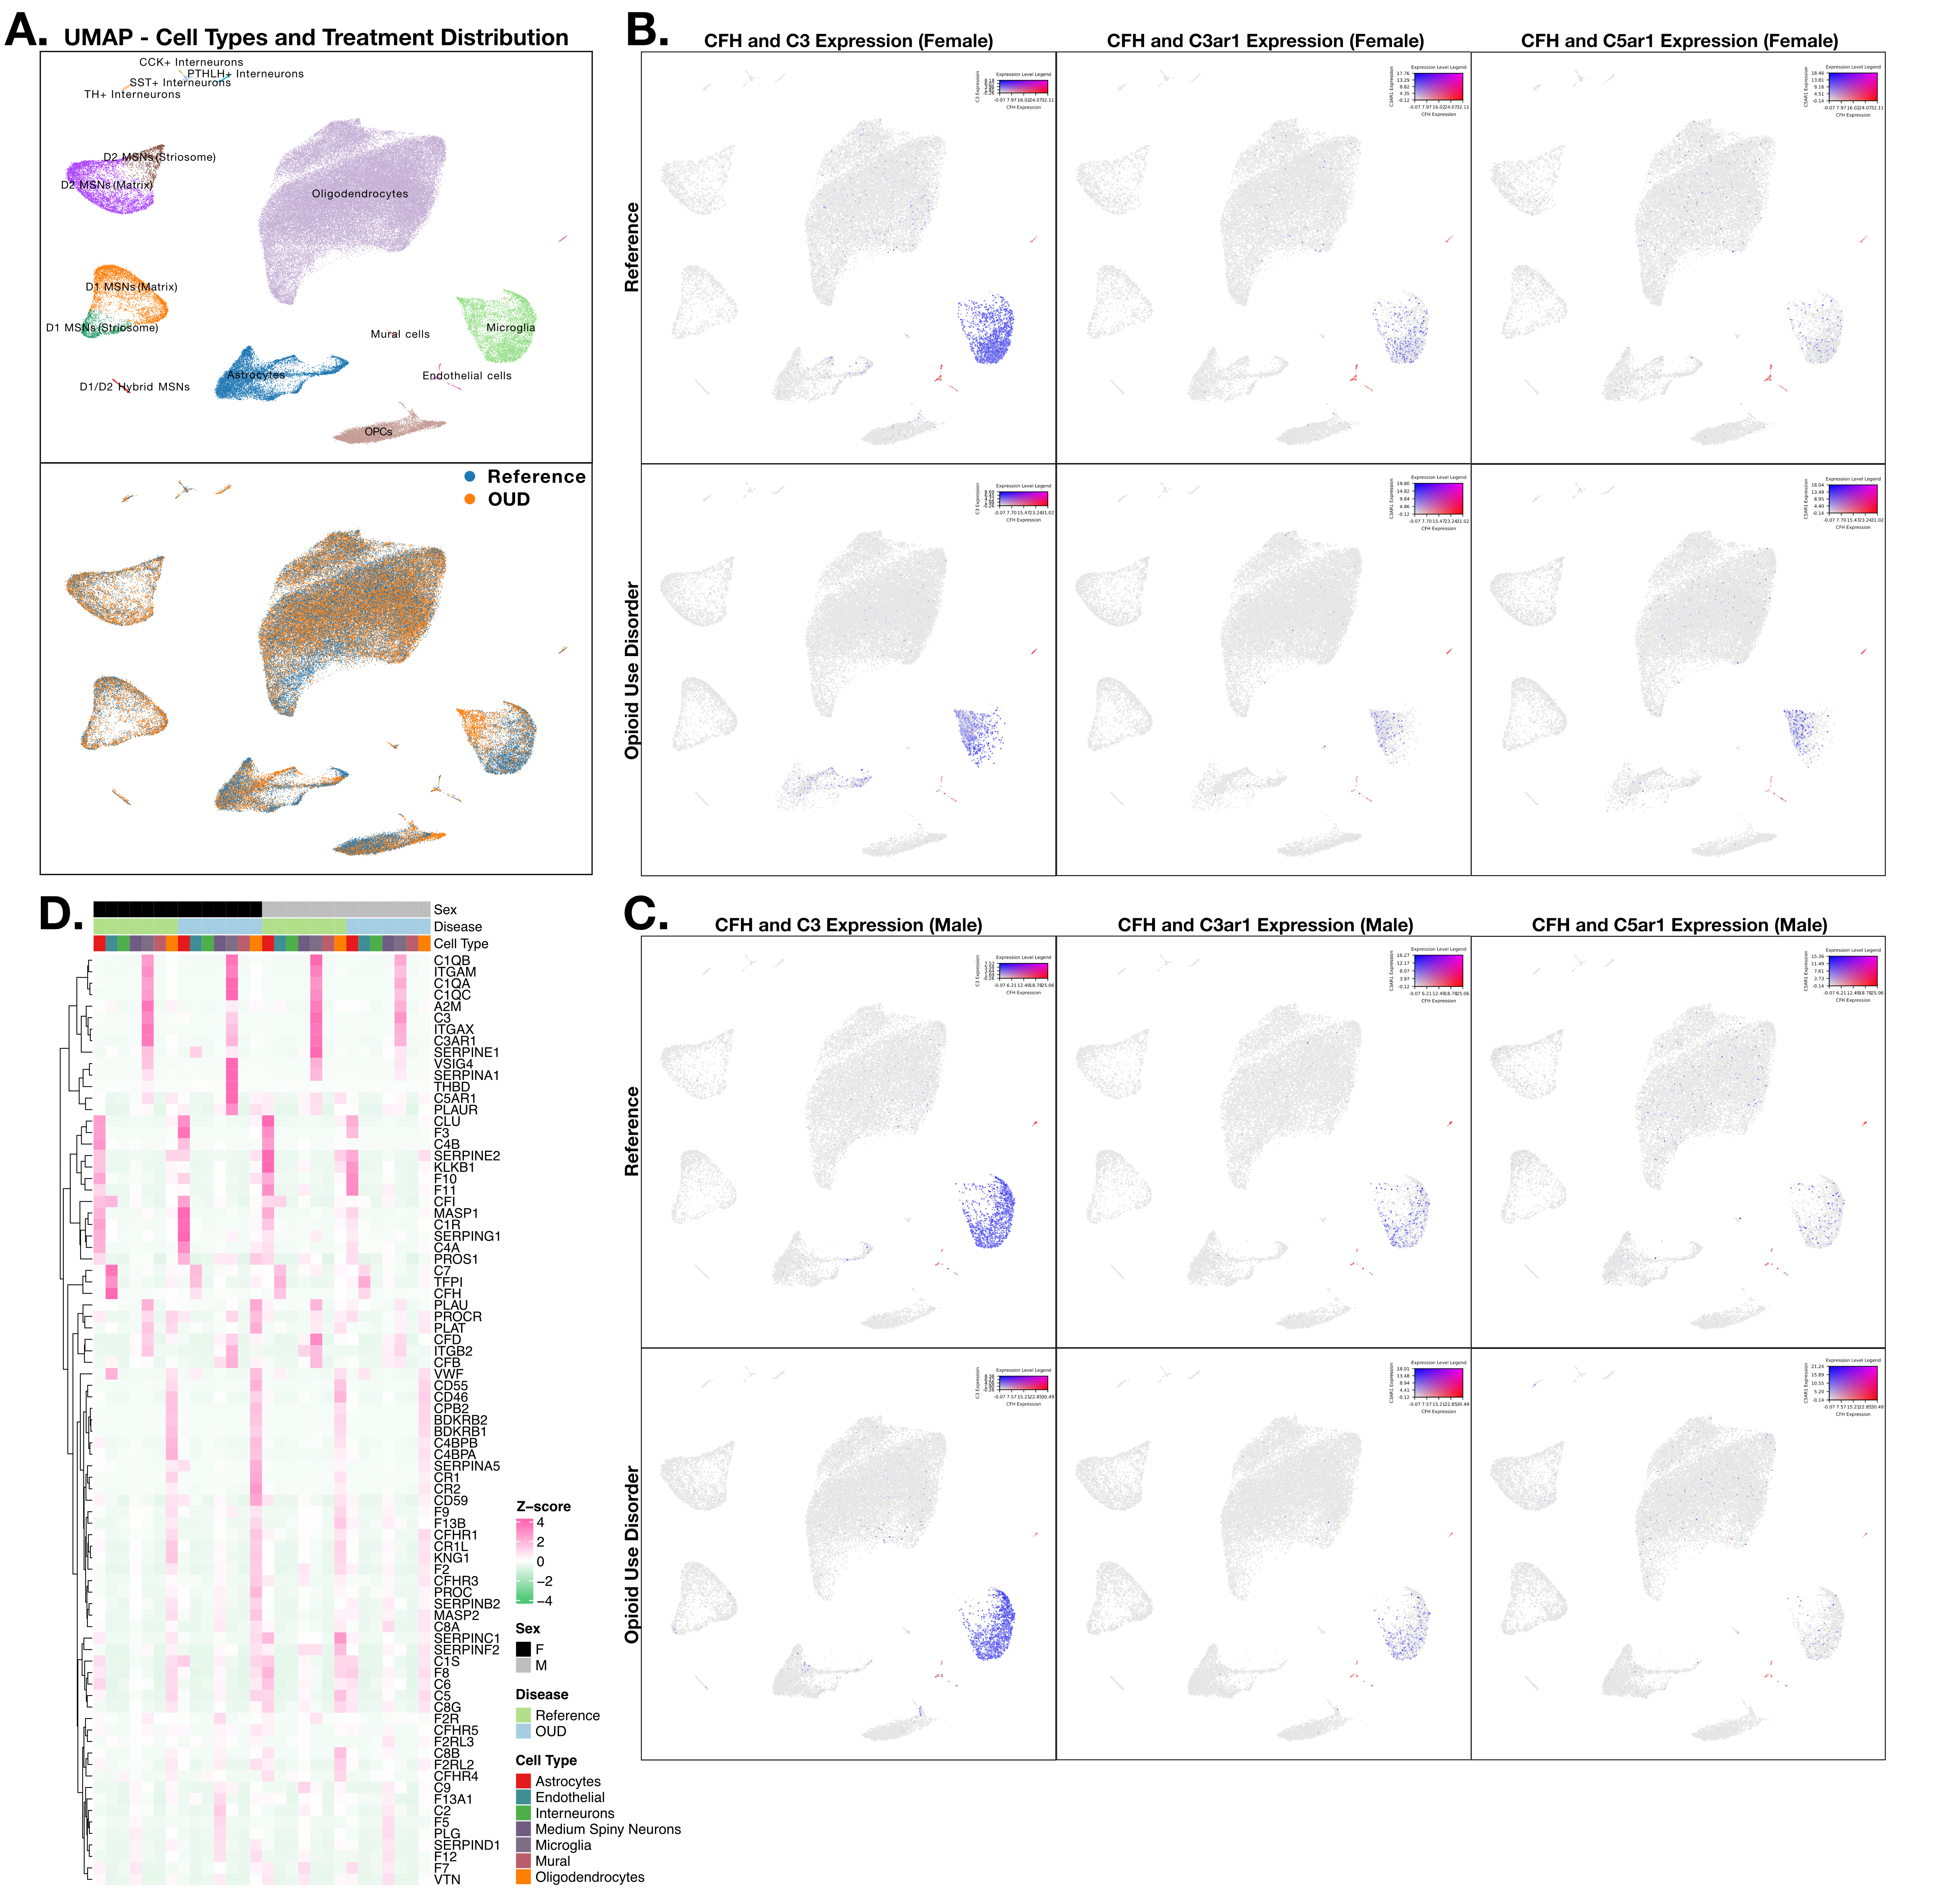
\includegraphics[width=1.00\textwidth]{Figure 1.jpg}
\caption{\color{Gray} \textbf{Visualization of Complement Expression in Human Brain.} 
Uniform Manifold Approximation and Projection (UMAP) and Heatmap visualizations of \texttt{GSE225158}. \textbf{A.} UMAP's depicting the distribution of cell types and treatments. \textbf{B.} UMAP visualizations showing expression of selected complement genes (CFH, C3aR1, C5aR1) in female samples (Reference \& OUD). CFH is expressed almost exclusively in the endothelial cells. C3, C3aR1, and C5aR1 are expressed primarily in the glial cells. C3, C3aR1, and C5aR1 expression shows large shifts between reference and OUD conditions in terms of which microglilal cells are expressing each respective gene \textbf{C.} Shows marginal changes in gene expression patterns. \textbf{D.} Heatmap plotting the expression of complement genes. Columns are organized by Sex, disease, and cell types| complement genes are primarily expressed in glial cells. Clustering of rows shows C3 and C1q's express in similar cells and at similar levels.
}
\label{Complement in Brain} % \label works only AFTER \caption within figure environment
\end{figure}

\subsection*{snRNA sequencing provides a map of complement proteins in healthy and OUD brains in both sexes.}
    Single-nucleus RNA sequencing (snRNA-seq) enabled us to map the cellular landscape of healthy and OUD-affected brains in both sexes. As illustrated in Fig \ref{Complement in Brain}A, we identified 11 distinct clusters (depicted in different colors), including astroglia, microglia, oligodendroglia, endothelial cells, mural cells, oligodendrocyte precursor cells (OPCs), and interneurons. Notably, the cell clusters from naïve and OUD brains largely overlapped, except for the OUD female group, where microglia were distinctly separated from their naïve counterparts.

\begin{figure}[ht] %s state preferences regarding figure placement here
%\renewcommand{\thefigure}{2}
% \centering
\includegraphics[width=1.00\textwidth]{Figure 2.jpg}
\caption{\color{Gray} \textbf{Exploring Transcription Factor Activity and Pathway Enrichment. } 
Sex dependent changes in transcription factor (TF) activity and pathway enrichment. \textbf{A.} Females show primarily increased activity of TFs, males show decreased activity of TFs. \textbf{B.} Pathway enrichment data from glial cells. Sexes show a distinct opposite enrichment of pathways.
}
\label{TF and Pathways} % \label works only AFTER \caption within figure environment
\end{figure}

\subsection*{snRNA sequencing shows differential expression of complement proteins in females and males with OUD.}
    Further analysis revealed differential expression of complement proteins in both females and males with OUD. In Fig \ref{Complement in Brain}B,C, we mapped the expression of Factor H (FH), C1q, C3, C3aR1, and C5aR1 across brain cell types using UMAP clustering. FH was predominantly expressed in endothelial cells but showed a decrease in expression within OUD cells. Other complement genes were primarily localized within microglial cells; notably, C5aR1 expression increased in OUD, whereas C3 and C3aR1 levels remained unchanged.

    We also examined the differential expression of transcription factors (Fig \ref{TF and Pathways}A) and found a surprising trend: transcription factors decreased across the board in male individuals with OUD, while they increased in females. To identify relevant pathways associated with complement, we conducted an enrichment analysis, generating a heat map. Consistent with the transcription factor results, pathway enrichment analysis indicated that inflammatory and immune pathways were reduced in males but increased in females with OUD.

\begin{figure}[ht] %s state preferences regarding figure placement here
%\renewcommand{\thefigure}{2}
% \centering
\includegraphics[width=1.00\textwidth]{Figure 4.jpg}
\caption{\color{Gray} \textbf{Complement Gene Differencial Expression in NAc and DLPFC. } 
\textbf{A.} Volcano Plots of different contrasts (sex-dependent \& region-dependent) Males in the NAc show a distinct increase in differencially expressed genes compared to the other contrasts. \textbf{B.} Heatmap plotting the expression of complement genes. Columns are organized by Sex, disease, and region| the NAc shows a upregulation of C1qa, C3, C3aR1, and C5 in both control and OUD conditions compared to an overall downregulation in the DLPFC for both conditions.
}
\label{VolcanoHeat} % \label works only AFTER \caption within figure environment
\end{figure}

\begin{figure}[ht]%s state preferences regarding figure placement here
%\renewcommand{\thefigure}{2}
% \centering
\includegraphics[width=1.00\textwidth]{Figure 3.jpg}
\caption{\color{Gray} \textbf{Complement Gene Expression in NAc and DLPFC. } 
This figure shows the regional distribution of C1qa, C1qb, C1qc, C3, C3aR1, C4A, C5, C5aR1, and CFH expression (log2 CPM) across different brain regions, faceted by sex and diagnosis. Each panel represents a specific demographic group (Male Control, Male OUD, Female Control, Female OUD). The boxplots display median and interquartile range of expression values, with individual data points representing individual samples. Statistical significance between brain regions within each demographic group was assessed using Wilcoxon rank-sum tests with Benjamini-Hochberg correction (*$p<0.05$, **$p<0.01$, ***$p<0.001$, ns: not significant).
}
\label{Box Plots} % \label works only AFTER \caption within figure environment
\end{figure}

\begin{figure}[ht]%s state preferences regarding figure placement here
%\renewcommand{\thefigure}{2}
% \centering
\includegraphics[width=1.00\textwidth]{Figure 5.jpg}
\caption{\color{Gray} \textbf{Complement Gene Expression in NAc and DLPFC. } 
This figure depicts the log2 CPM expression levels of C3, C4A, C5, and CFH across different brain regions in individuals with and without opioid use disorder (OUD). Expression data is grouped by sex (Male/Female) and diagnosis (Control/OUD), with separate panels for each brain region. Boxplots show the median and interquartile range, with individual data points representing individual samples. Statistical significance between groups was determined using Wilcoxon rank-sum tests with Benjamini-Hochberg correction for multiple comparisons (*$p<0.05$, **$p<0.01$, ***$p<0.001$, ns: not significant).
}
\label{Box Plots2} % \label works only AFTER \caption within figure environment
\end{figure}

\subsection*{snRNA sequencing shows differential expression of complement proteins and transcription factors, while bulk RNA seq shows no changes with OUD.}
    To determine whether the snRNA-seq findings were reflected in bulk RNA sequencing data, we queried the publicly available dataset (GSE174409) from the dorsolateral prefrontal cortex and nucleus accumbens. The results were represented in box plots (Figure \ref{Box Plots}), volcano plots and heatmaps (Figure \ref{VolcanoHeat}); we find that the bulk RNA data lines up with our findings from the snRNA-seq data. The box plots (Figure \ref{Box Plots}) show significant changes in C3, C4A, and C5 expression across regions| we see for each that the NAc has a higher level of expression of each gene regardless of disease or sex. This prompted us to look at if sex and disease played a role in this significance as well (Figure \ref{Box Plots2}) shows that this is not the case. Rather, figure \ref{Box Plots2} shows that these genes are differentially expressed in a region specific manner with no significant influence of sex and disease.

%\clearpage makes sure that all above content is printed at this point and does not invade into the upcoming content
%\clearpage

\section*{Discussion}

In summary, our study utilized publicly available single-cell and bulk RNA sequencing data to assess the differential expression of complement genes between males and females as well as between naïve individuals and those with OUD. Our findings indicate that complement protein expression significantly changes in the context of OUD, with notable differences observed between sexes. This aligns with our previous study, which demonstrated alterations in complement protein expression in the brains of individuals with HIV and OUD. Importantly, our current results suggest that the response of complement proteins varies by sex, underscoring the need for tailored treatment approaches.
We confirmed that Factor H is predominantly expressed in endothelial cells, consistent with previous findings, and demonstrated that FH expression is reduced in OUD. This reduction could contribute to enhanced complement activation and its downstream effects, implicating FH as a key player in the pathology of OUD.
While our study focused on inflammatory and immune pathways, the complement field is rapidly evolving, revealing novel functions for complement proteins that warrant further investigation. Future studies should explore the pathways impacted by complement proteins in this context and their potential effects on clinical treatments. Given the significant physiological differences between human and mouse brains at the cellular level, our work is crucial for understanding the relevance of mouse models.
A comprehensive understanding of cellular heterogeneity in the brain is essential for the development of effective therapies. The efficacy of targeting specific complement proteins will depend on the cell-type-specific expression and activity of associated pathways. Our study represents an initial step toward this important goal.


\subsection*{Limitations of This Study}
Our study has limitations that must be acknowledged. Firstly, we did not perform in vitro or in vivo validation of the computed metamarkers. Secondly, we did not substantiate the observed transcriptional changes at the protein level. Additionally, our analysis did not encompass all cell types in the brain, as supervised cell classification remains challenging due to the lack of precise definitions for cell types, insufficient robust markers, technical limitations, and sampling variability. Moreover, neural plasticity and the ability of cells to change type may lead to the emergence of less-defined cellular populations.
Furthermore, due to the small sample size, we are unable to establish direct links between variations in cellular composition and specific disease features, such as disease phenotypes, drug responsiveness, or long-term prognosis. Thus, evaluating the clinical relevance of our findings will necessitate a larger cohort or access to additional datasets with comprehensive associated metadata, which is currently not available.



%\clearpage

% \section*{Supporting Information}
% If you intend to keep supporting files separately you can do so and just provide figure captions here. Optionally make clicky links to the online file using \verb!\href{url}{description}!.

% %These commands reset the figure counter and add "S" to the figure caption (e.g. "Figure S1"). This is in case you want to add actual figures and not just captions.
% \setcounter{figure}{0}
% \renewcommand{\thefigure}{S\arabic{figure}}

% % You can use the \nameref{label} command to cite supporting items in the text.
% \subsection*{S1 Figure}
% \label{example_label}
% {\bf Caption of Figure S1.} \textbf{A}, If you want to reference supporting figures in the text, use the \verb!\nameref{}!. command. This will reference the section's heading: \nameref{example_label}.

% \subsection*{S2 Video}
% \label{example_video}
% {\bf Example Video.} Use \href{www.youtube.com}{clicky links} to the online sources of the files.

% %\clearpage

% \section*{Acknowledgments}
% We thank just about everybody.

\nolinenumbers

%This is where your bibliography is generated. Make sure that your .bib file is actually called library.bib
\bibliography{library}

%This defines the bibliographies style. Search online for a list of available styles.
\bibliographystyle{abbrv}

\end{document}